%%%%%%%%%%%%%%%%%%%%%%%%%%%%%%%%%%%%%%%%%%%%%%%%%%%%%%%%%%%
% --------------------------------------------------------
% Informe de Laboratorio -- Visión Artificial
% Máster en Inteligencia Artificial -- UNIR
%
% Plantilla basada en Rho-class v3.0.1
% Autor original: Guillermo Jimenez (memo.notess1@gmail.com)
% Licencia: Creative Commons CC BY 4.0
% --------------------------------------------------------
%%%%%%%%%%%%%%%%%%%%%%%%%%%%%%%%%%%%%%%%%%%%%%%%%%%%%%%%%%%

\documentclass[12pt,a4paper,twoside]{rho-class/rho}
\usepackage[spanish,es-nodecimaldot,es-noindentfirst]{babel}
\usepackage{booktabs}
\usepackage{setspace}
\usepackage[section]{placeins}
\setstretch{1.5}
\setlength{\textfloatsep}{16pt plus 3pt minus 3pt}
\setlength{\floatsep}{14pt plus 3pt minus 3pt}

%----------------------------------------------------------
% Tipo de documento
%----------------------------------------------------------

\doctype{Informe de Laboratorio}
\title{Mejora de Imagen: operaciones elementales}

%----------------------------------------------------------
% Autor, Afiliación y Fechas
%----------------------------------------------------------

\author[a,1]{Javier Gallego Fernández}

\affil[a]{Máster en Inteligencia Artificial, Universidad Internacional de La Rioja (UNIR)}

%----------------------------------------------------------
% Información del autor y del documento
%----------------------------------------------------------

\corres{\textsuperscript{1}Autor: \href{mailto:javgalfer@gmail.com }{javgalfer@gmail.com }}

% \docinfo{Informe elaborado en el marco de la asignatura Visión Artificial del Máster en Inteligencia Artificial de la UNIR.}

%----------------------------------------------------------

\journalname{UNIR}
\journal{Visión Artificial}
\theday{\today}
\vol{1}
\no{1}

%----------------------------------------------------------
% Resumen y palabras clave
%----------------------------------------------------------

\begin{abstract}
    Se diseñó y evaluó un flujo de mejora de imagen para
    un conjunto de cuatro fotografías nocturnas con baja iluminación extraídas del
    conjunto de datos \textit{DARK FACE}~\parencite{yang2020darkface}. Para la imagen de
    mayor oscuridad y menos puntos de luz se aplicó la ley de potencia ($\gamma = 0{,}40$), 
    aprovechando que valores de gamma menores que 1 expanden el rango de intensidad de los píxeles más oscuros. En las otras tres imágenes,
    con fuentes de luz y un mayor rango dinámico, se aplicó una transformación logarítmica. Esta permite mapear un rango pequeño de valores en un rango más amplio, por lo que es muy efectiva para realzar zonas con baja iluminación sin saturar las más iluminadas.
    En todas ellas, se aplicó posteriormente Ecualización Adaptativa de Histograma con Limitación de Contraste (CLAHE) sobre el canal~$L^*$ (CLAHE LAB) para mejorar el contraste localmente sin sobrecargarlo globalmente.
    La validación mediante histogramas y funciones de distribución acumulada (CDF) mostró un mayor grado de dispersión y un perfil de intensidad más uniforme.
\end{abstract}

\keywords{mejora de imágenes, CLAHE, ley de potencia, transformación logarítmica, visión artificial}

%----------------------------------------------------------

\begin{document}

%----------------------------------------------------------
% Portada
%----------------------------------------------------------

\onecolumn
\begin{titlepage}
    \begin{center}
        \vspace*{2.5cm}
        {\large\sffamily Universidad Internacional de La Rioja}\\[0.3em]
        {\large\sffamily Máster en Inteligencia Artificial}\\[3cm]
        {\LARGE\bfseries\sffamily Mejora de Imagen: operaciones elementales}\\[1.2cm]
        {\large\sffamily\itshape Informe de Laboratorio\\[0.3em]
        Asignatura: Visión Artificial}\\[3.5cm]
        {\normalsize\sffamily
        \begin{tabular}{rl}
            Alumno:  & Javier Gallego Fernández \\[0.3em]
            Fecha:   & \today          \\
        \end{tabular}}
    \end{center}
\end{titlepage}

%----------------------------------------------------------
% Índice
%----------------------------------------------------------

\tableofcontents
\newpage

%----------------------------------------------------------
% Inicio del artículo (una columna)
%----------------------------------------------------------

\maketitle
\thispagestyle{firststyle}

%----------------------------------------------------------

\section{Introducción}

    \rhostart{L}a mejora de imágenes es una de las etapas más importantes del procesamiento de imágenes, ayudando a mejorar la calidad, la interpretabilidad y a facilitar la extracción de información relevante. Su relevancia abarca disciplinas como la medicina (para la identificación de patologías) o la visión por computador (para delimitar bordes de objetos).

    El preprocesamiento se encuentra en las primeras etapas de tratamiento, 
    actuando como un conjunto de transformaciones destinadas a capturar la información relevante 
    de la imagen frente a la menos relevante. En escenas de baja iluminación como las que se abordan en este artículo, donde los valores de intensidad se concentran en  un rango menor,
    esta etapa es especialmente crítica, ya que la información se encuentra comprimida, lo que dificulta su interpretación tanto por parte de observadores como de siguientes fases de procesamiento.

    Las técnicas examinadas en este artículo, la ley de potencia, la transformación
    logarítmica y el procesado del histograma (mediante CLAHE), son técnicas que permiten aumentar el nivel de contraste de la imagen. Expanden el rango de intensidad de los píxeles oscuros y logran una mayor dispersión tendiendo a un perfil más uniforme. 
    Estas técnicas son las que mejor han funcionado con el conjunto de imágenes nocturnas.

%----------------------------------------------------------

\section{Material y métodos}

    \subsection{Entorno de trabajo y conjunto de imágenes}

        El procesamiento se realizó en un entorno Python~3.14 con las librerías
        OpenCV~4, NumPy y Matplotlib para el tratamiento de las imágenes y la visualización de resultados. El código
        completo se realizó en un cuaderno Jupyter Notebook, para facilitar la reproducibilidad de los resultados y las pruebas iterativas de parámetros.

        El conjunto de imágenes son cuatro fotografías nocturnas extraídas
        del conjunto de datos \textit{DARK FACE}~\parencite{yang2020darkface}, cuyo
        propósito original es el estudio de la detección de rostros en condiciones
        de baja iluminación. Las imágenes, identificadas como 1187.png, 1321.png,
        1457.png y 1619.png, presentan una resolución de 1080 x 720 píxeles,
        profundidad de color de 8~bits por canal y codificación en tres canales RGB.
        Las escenas corresponden a exteriores nocturnos con alto
        contenido de sombras y fuentes de luz puntuales, lo que las convierte en casos de estudio ideales para evaluar técnicas de mejora de imagen orientadas a la recuperación de detalles en zonas oscuras.

    \subsection{Técnicas de mejora aplicadas}

        Se emplearon tres técnicas de mejora de imagen, seleccionadas en función de
        las características de cada imagen.

        \textbf{Ley de potencia.} La función
        $s = c \cdot r^{\gamma}$, con $c = 255^{1-\gamma}$ para normalizar la
        salida al rango $[0, 255]$ y $\gamma < 1$, que expande los píxeles oscuros
        comprimiendo los claros~\parencite{huang2013agcwd}. El valor de $\gamma$ se seleccionó realizando pruebas y visualizando el resultado, buscando un equilibrio entre la visibilidad en zonas oscuras y la saturación en las más iluminadas.
        Para la imagen~1187, cuya distribución de
        intensidades se concentra casi íntegramente por debajo de 20, se
        seleccionó $\gamma = 0{,}40$ con el fin de recuperar estructura en las
        regiones más oscuras sin saturar las pocas zonas ya iluminadas.

        \textbf{Transformación logarítmica.} La función
        $s = c \cdot \log_{10}(1 + r)$, con $c = 255 / \log_{10}(256)$ para
        normalizar la salida al rango $[0, 255]$, se emplea para expandir de 
        forma no lineal las intensidades bajas y comprimir simultáneamente las altas. 
        Esta propiedad la hace más adecuada que la ley de potencia en escenas oscuras 
        con puntos de luz intensos, ya que permite realzar el detalle en 
        sombras sin saturar las luces~\parencite{drago2003logmapping}. Por este motivo, se seleccionó como
        primera etapa de procesamiento para las imágenes~1321, 1457 y~1619.

        \textbf{Ecualización adaptativa de histograma con limitación de contraste
        (CLAHE).} A diferencia de la ecualización global de histograma, CLAHE
        opera localmente sobre regiones de la imagen (\textit{tiles}) y limita la
        ganancia máxima mediante un umbral de recorte (\textit{clip limit}),
        evitando la amplificación del ruido~\parencite{zuiderveld1994clahe}. Para no alterar la cromaticidad, CLAHE se
        aplicó exclusivamente sobre el canal~$L^*$ del espacio de color CIE-Lab,
        con los parámetros (\textit{clip limit})\,=\,2{,}0 y (\textit{tile grid size})\,=\,8 x 8 para
        todas las imágenes. De nuevo, se fueron probando diferentes combinaciones de parámetros que mejorasen la imagen sin introducir ruido excesivo.

    \subsection{Procedimiento experimental}

        Para todas las imágenes, el flujo de procesamiento aplicado a cada imagen consta de las cuatro
        etapas siguientes.

        \begin{enumerate}
            \item \textbf{Análisis de la imagen original.} Se cargó cada imagen en
            formato RGB y se inspeccionó su histograma en los canales RGB y en
            escala de grises.

            \item \textbf{Ajuste de intensidad.} Para la
            imagen~1187 se aplicó la ley de potencia con $\gamma = 0{,}40$; para las
            imágenes~1321, 1457 y~1619 se aplicó la transformación logarítmica
            normalizada. Esta etapa tiene como propósito redistribuir la información de luminancia hacia un rango
            de intensidades más amplio y más uniforme.

            \item \textbf{Procesado del histograma.} Sobre la imagen
            resultante del paso anterior se aplicó CLAHE en el espacio CIE-Lab,
            actuando exclusivamente sobre el canal~$L^*$, con
            (\textit{clip limit})\,=\,2{,}0 y (\textit{tile grid size})\,=\,8 x 8. Esta etapa permitió
            mejorar el contraste local sin amplificar el ruido de manera global, revelando detalles de textura 
            que no eran perceptibles en la imagen original ni tras el ajuste de intensidad.

            \item \textbf{Validación.} La evaluación comparando cada etapa del flujo (original,
            ajuste de intensidad y procesado del histograma). Se visualizaron histogramas y funciones de
            distribución acumulada (CDF) para cada imagen, permitiendo valorar
            de manera cualitativa el efecto de cada transformación sobre la
            distribución.
        \end{enumerate}

%----------------------------------------------------------

\section{Resultados}

    Para cada imagen se presentan la comparativa visual de las tres etapas
    del flujo (original, ajuste de intensidad y procesado del histograma), junto con los histogramas del
    canal~$L^*$ y sus funciones de distribución acumulada (CDF).

    \subsection{Imagen 1187: Ley de potencia + CLAHE LAB}

        La imagen~1187 presentaba la distribución de intensidades más concentrada
        en el extremo oscuro del conjunto, con prácticamente todos los
        píxeles próximos a 0. Como se aprecia en la Figura~\ref{fig:1187_visual},
        la ley de potencia con $\gamma = 0{,}40$ produce una expansión del rango que
        recupera estructura visible en regiones con muy poca luminancia. También se observa saturación en los
        bordes de la imagen, una
        limitación inherente al uso de valores de gamma muy bajos en imágenes con
        rango dinámico reducido. La aplicación
        posterior de CLAHE LAB atenúa un poco este efecto al limitar la
        ganancia local. Como muestra la Figura~\ref{fig:1187_hist}, el histograma resultante presenta una
        redistribución hacia valores medios-altos y una CDF más próxima a la
        diagonal, indicativa de mayor aprovechamiento del rango dinámico
        disponible.

        \begin{figure}[t]
            \centering
            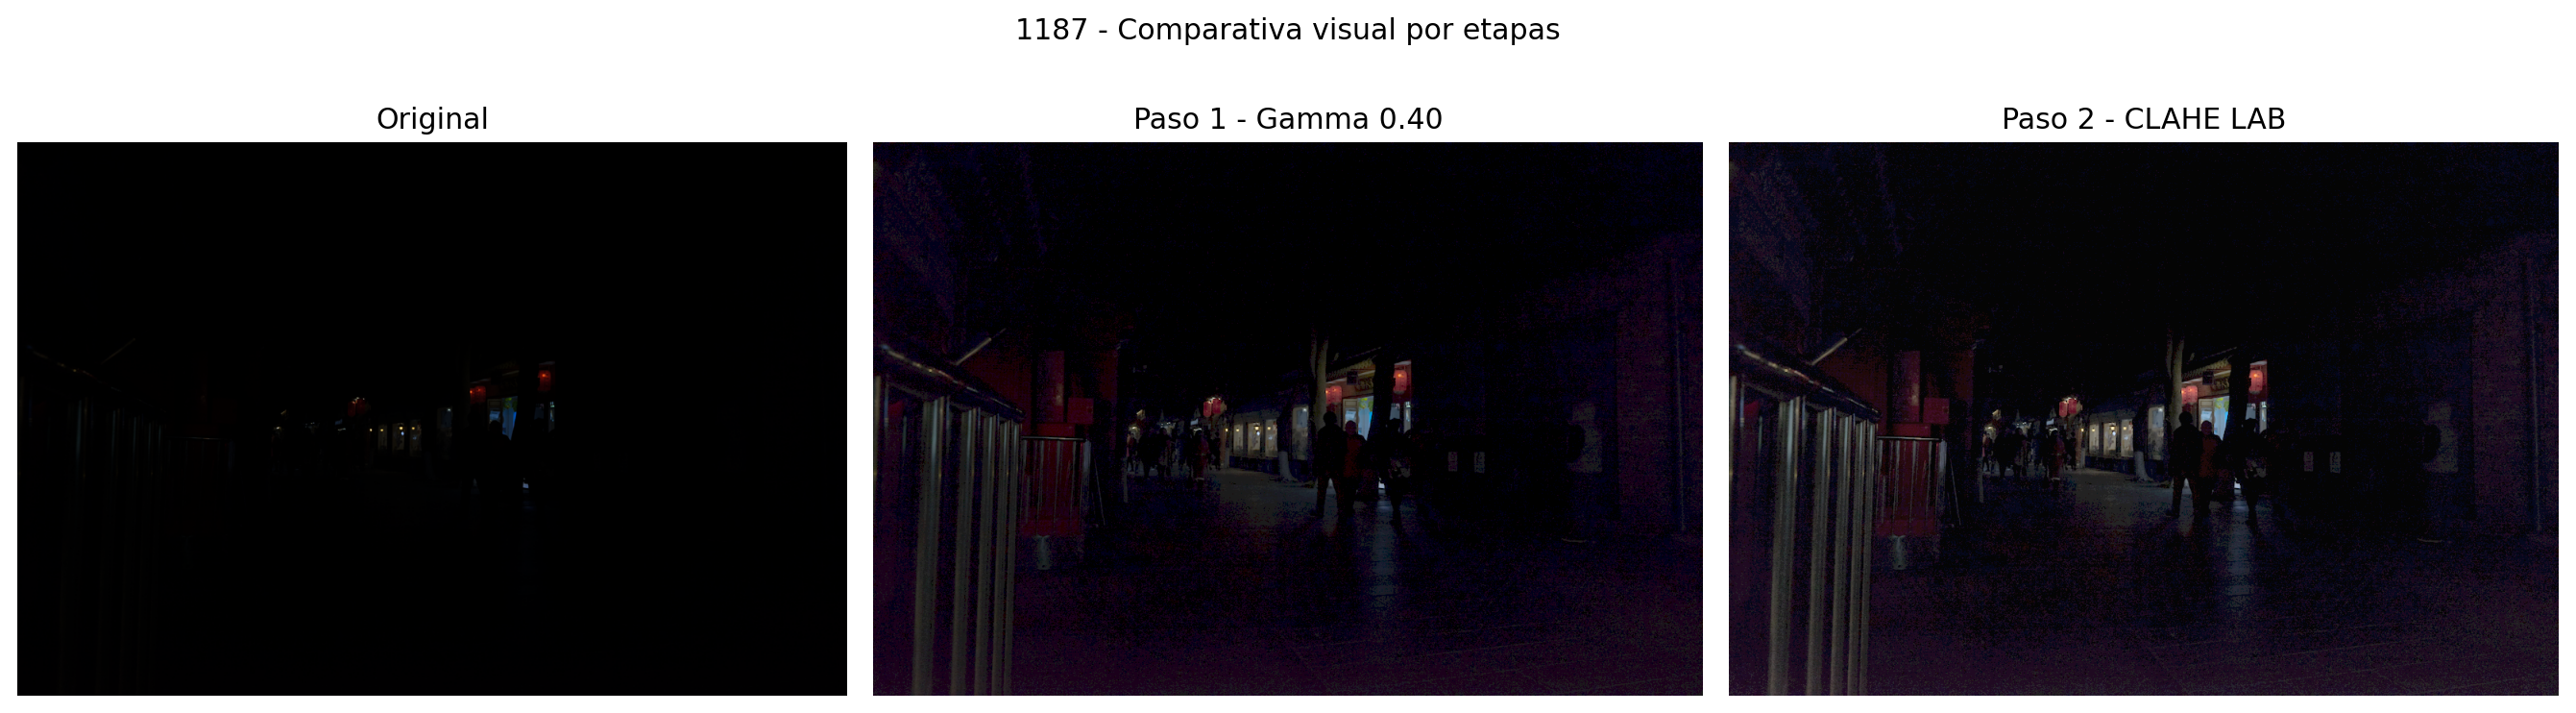
\includegraphics[width=\textwidth]{figures/fig_1187_visual.png}
            \caption{Imagen~1187: comparativa visual por etapa. De izquierda a
            derecha: original, ley de potencia, $\gamma = 0{,}40$ y
            CLAHE LAB, clip\,=\,2{,}0, tile\,=\,$8\times8$.}
            \label{fig:1187_visual}
        \end{figure}

        \begin{figure}[t]
            \centering
            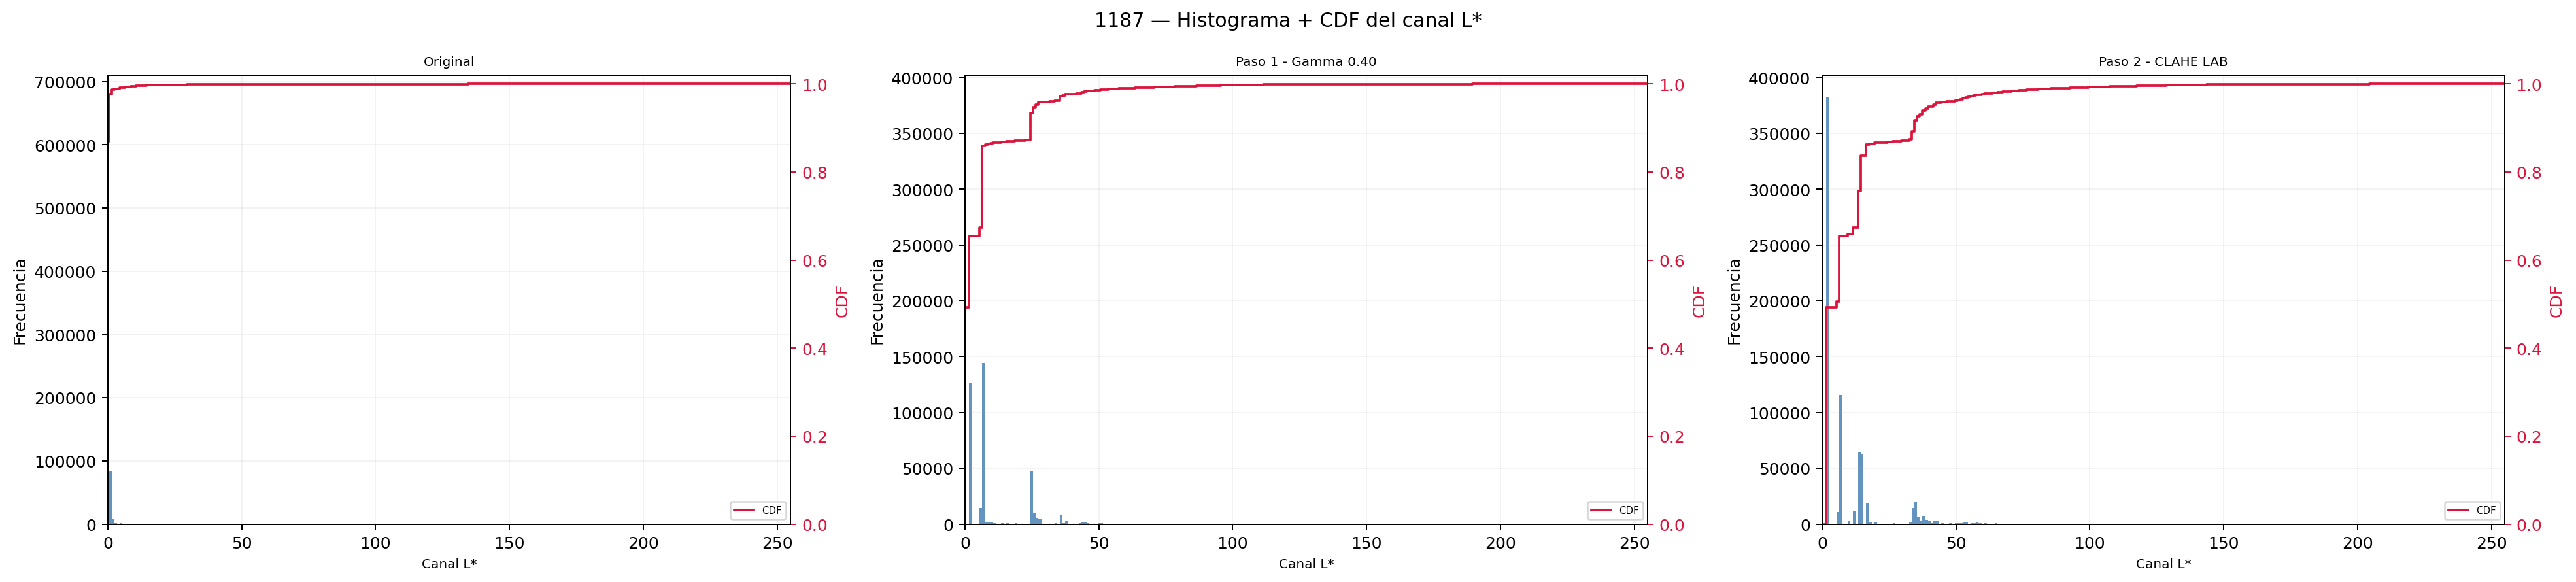
\includegraphics[width=\textwidth]{figures/fig_1187_hist.png}
            \caption{Imagen~1187: histogramas y CDF del
            canal~$L^*$ para cada etapa del flujo.}
            \label{fig:1187_hist}
        \end{figure}

    \subsection{Imagen 1321: Transformación Logarítmica + CLAHE LAB}

        Como se observa en la Figura~\ref{fig:1321_visual}, la transformación logarítmica aplicada a la imagen~1321 produce un
        realce progresivo que comprime el rango dinámico en mayor medida que la
        ley de potencia, siendo especialmente efectiva para expandir el rango
        útil en imágenes con una distribución dominada por píxeles oscuros pero
        con presencia de zonas de iluminación media. Después, la aplicación de
        CLAHE LAB incrementa el contraste local de manera adaptativa. Sin
        embargo, la combinación de ambas técnicas puede introducir un grano fino
        visible en ciertas zonas, lo que es un efecto de aumento del ruido local.
        En la Figura~\ref{fig:1321_hist} se aprecia además el desplazamiento de la distribución hacia valores más altos y una CDF más uniforme.

        \begin{figure}[t]
            \centering
            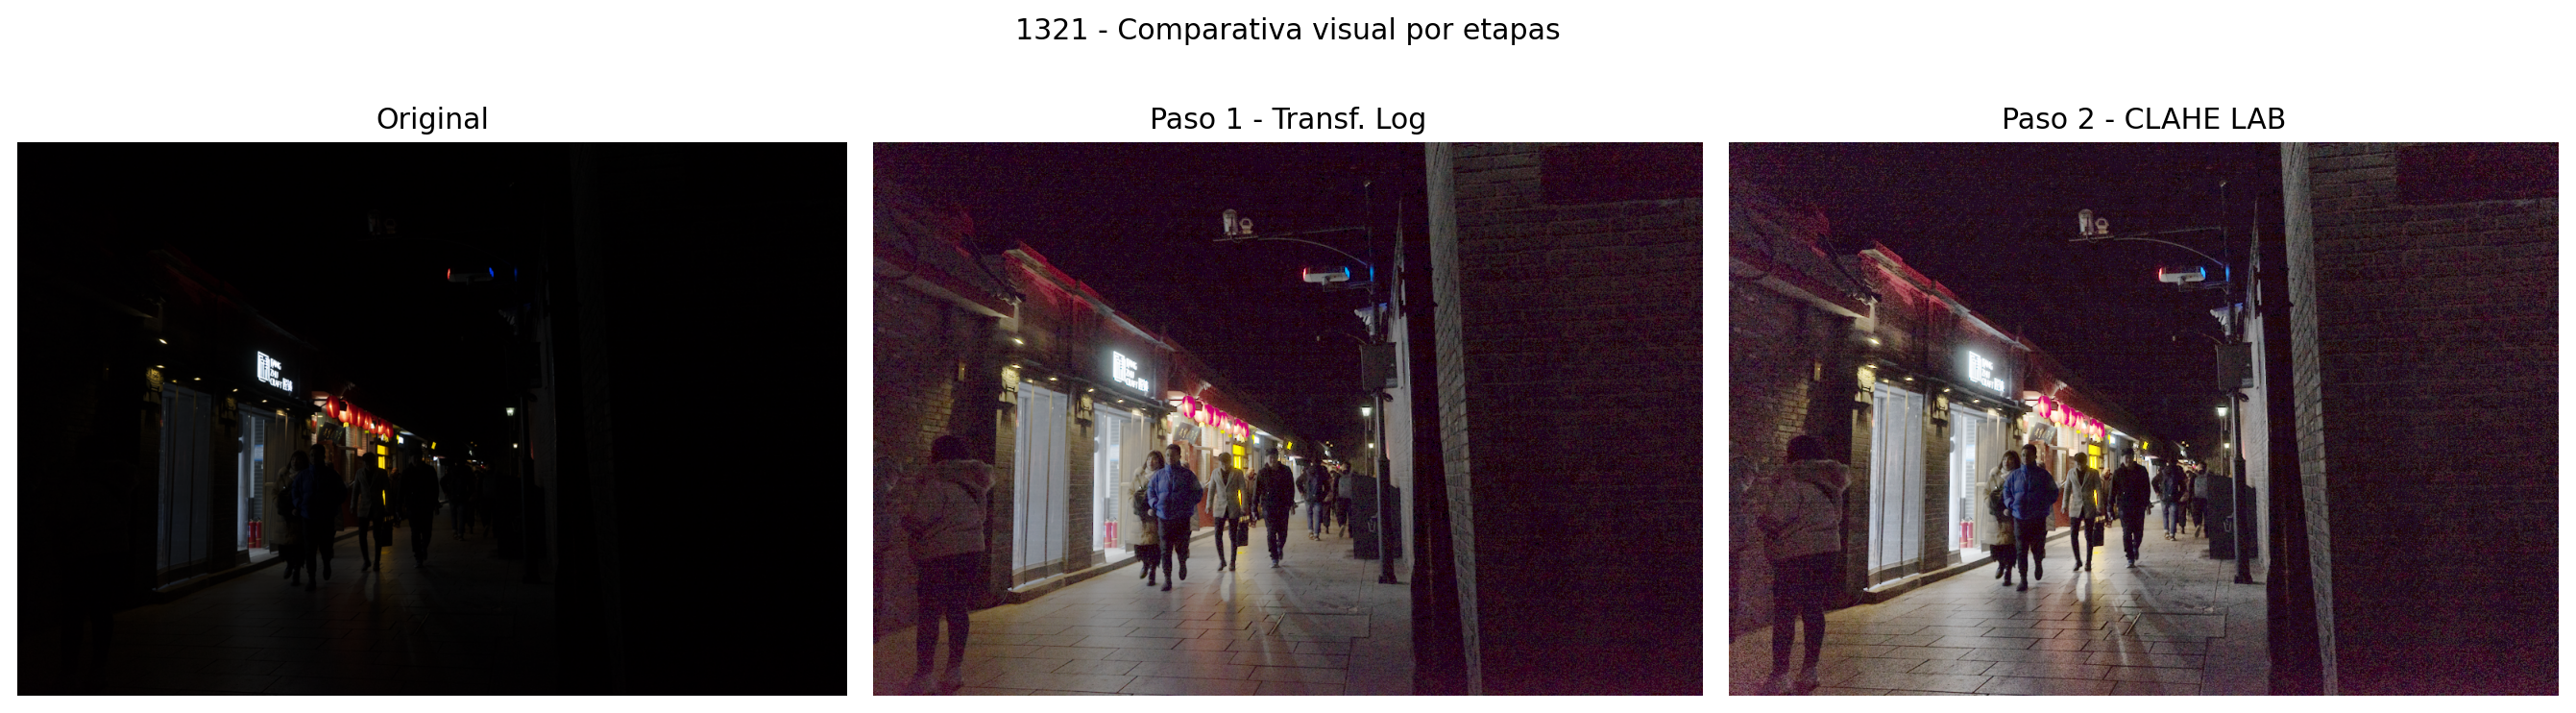
\includegraphics[width=\textwidth]{figures/fig_1321_visual.png}
            \caption{Imagen~1321: comparativa visual por etapa. De izquierda a
            derecha: original, transformación logarítmica y
            CLAHE LAB, clip\,=\,2{,}0, tile\,=\,$8\times8$.}
            \label{fig:1321_visual}
        \end{figure}

        \begin{figure}[t]
            \centering
            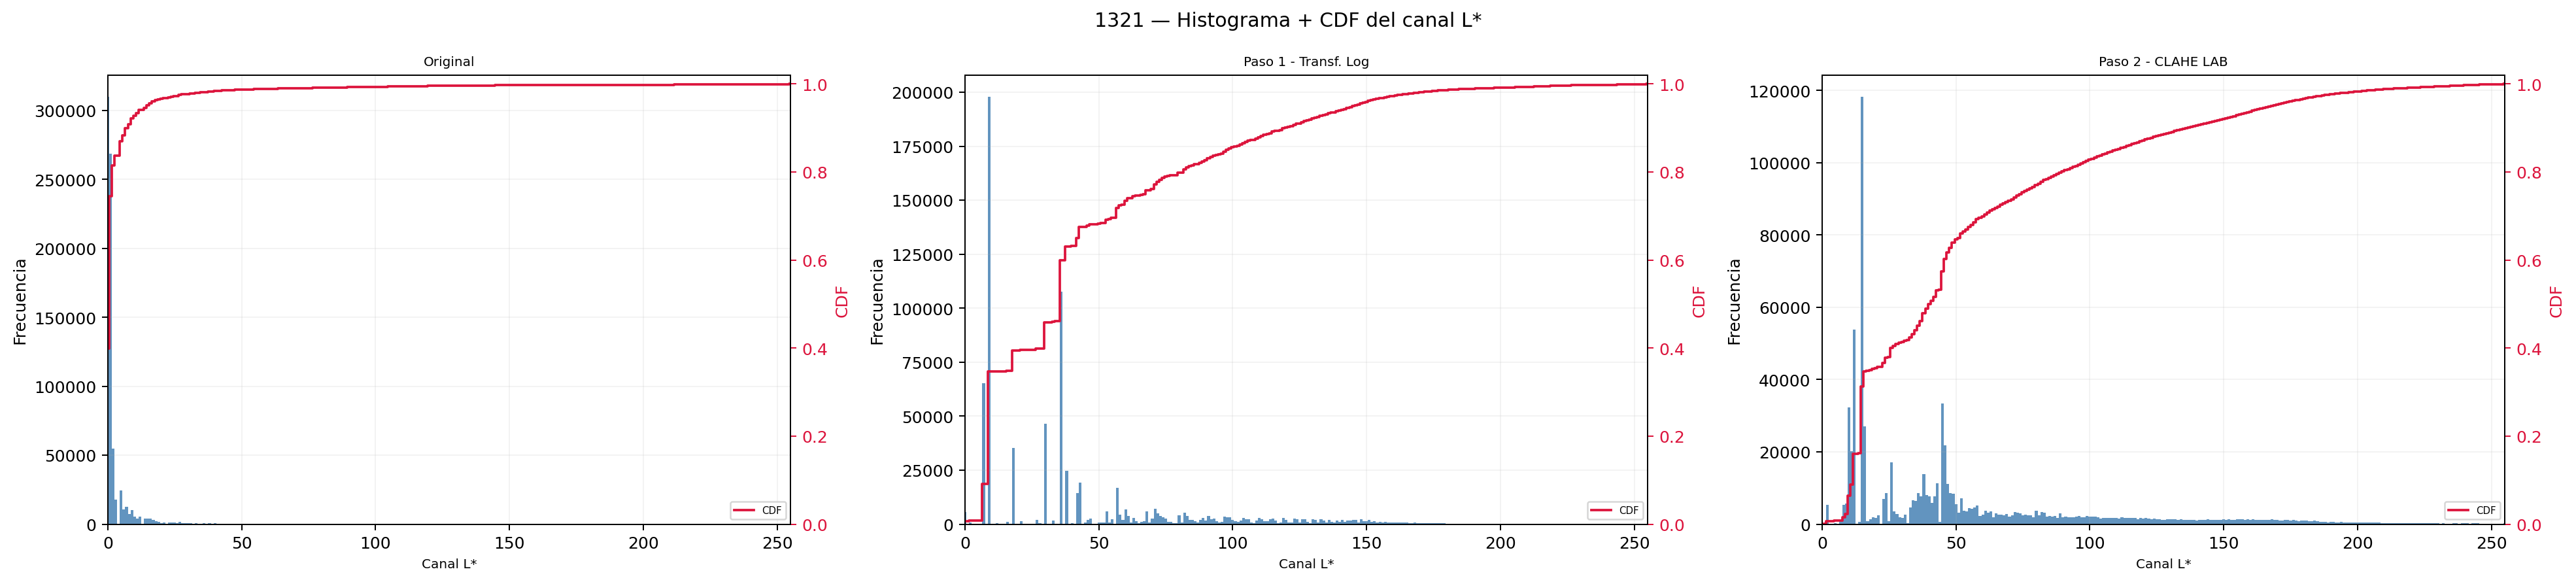
\includegraphics[width=\textwidth]{figures/fig_1321_hist.png}
            \caption{Imagen~1321: histogramas y CDF del canal~$L^*$ por etapa.}
            \label{fig:1321_hist}
        \end{figure}

    \subsection{Imagen 1457: Transformación Logarítmica + CLAHE LAB}

        La imagen~1457 presentaba unas condiciones de iluminación ligeramente
        superiores al resto (valores concentrados entre 0 y 25 pero con algunos picos más altos), lo que provocó que la transformación logarítmica,
        visible en la Figura~\ref{fig:1457_visual}, generase un realce más suave, pero también una cierta compresión del
        contraste global, dando lugar a una apariencia más clara. 
        La aplicación de CLAHE LAB compensa parcialmente este efecto al incrementar el contraste
        local, permitiendo recuperar detalles
        de textura en la calzada, el arbolado y el resto de elementos como edificios y coches.

        En cuanto a los histogramas, la Figura~\ref{fig:1457_hist} muestra que las mejoras aplicadas consiguen redistribuir las intensidades hacia un rango más uniforme. La curva de la CDF se acerca a la diagonal, lo que indica un mejor aprovechamiento del rango dinámico disponible.

        \begin{figure}[t]
            \centering
            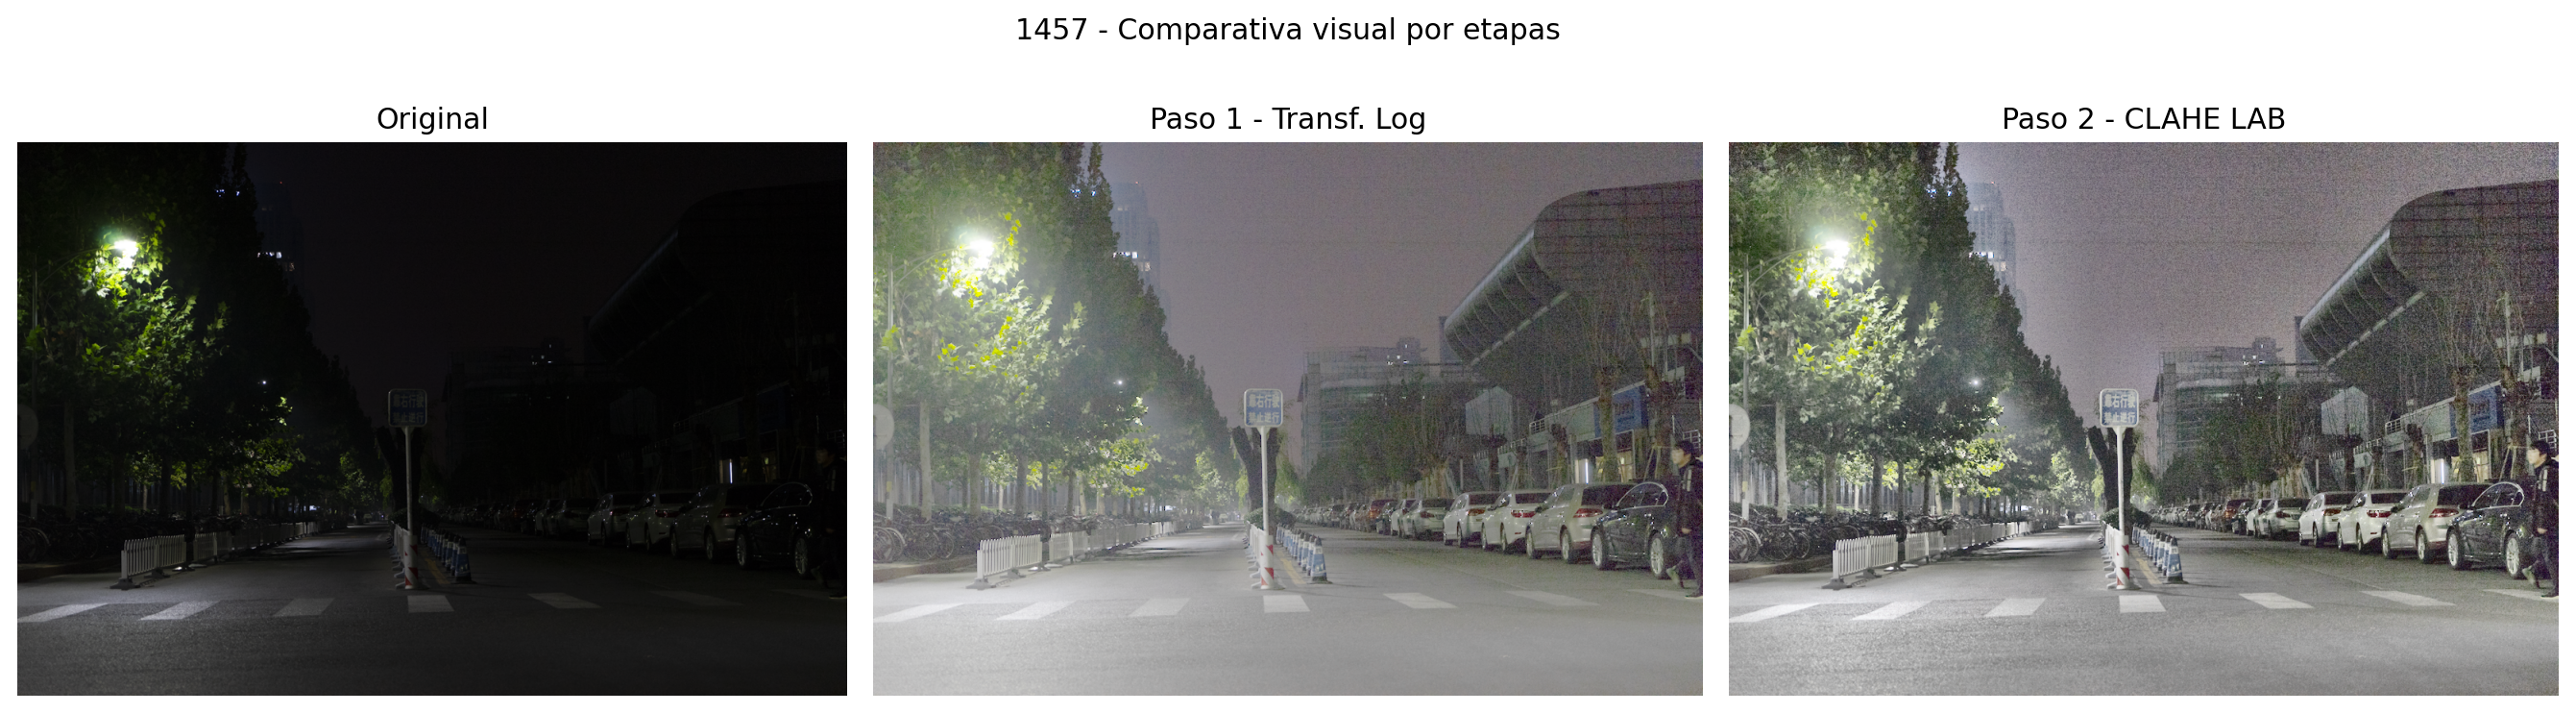
\includegraphics[width=\textwidth]{figures/fig_1457_visual.png}
            \caption{Imagen~1457: comparativa visual por etapa. De izquierda a
            derecha: original, transformación logarítmica y
            CLAHE LAB, clip\,=\,2{,}0, tile\,=\,$8\times8$.}
            \label{fig:1457_visual}
        \end{figure}

        \begin{figure}[t]
            \centering
            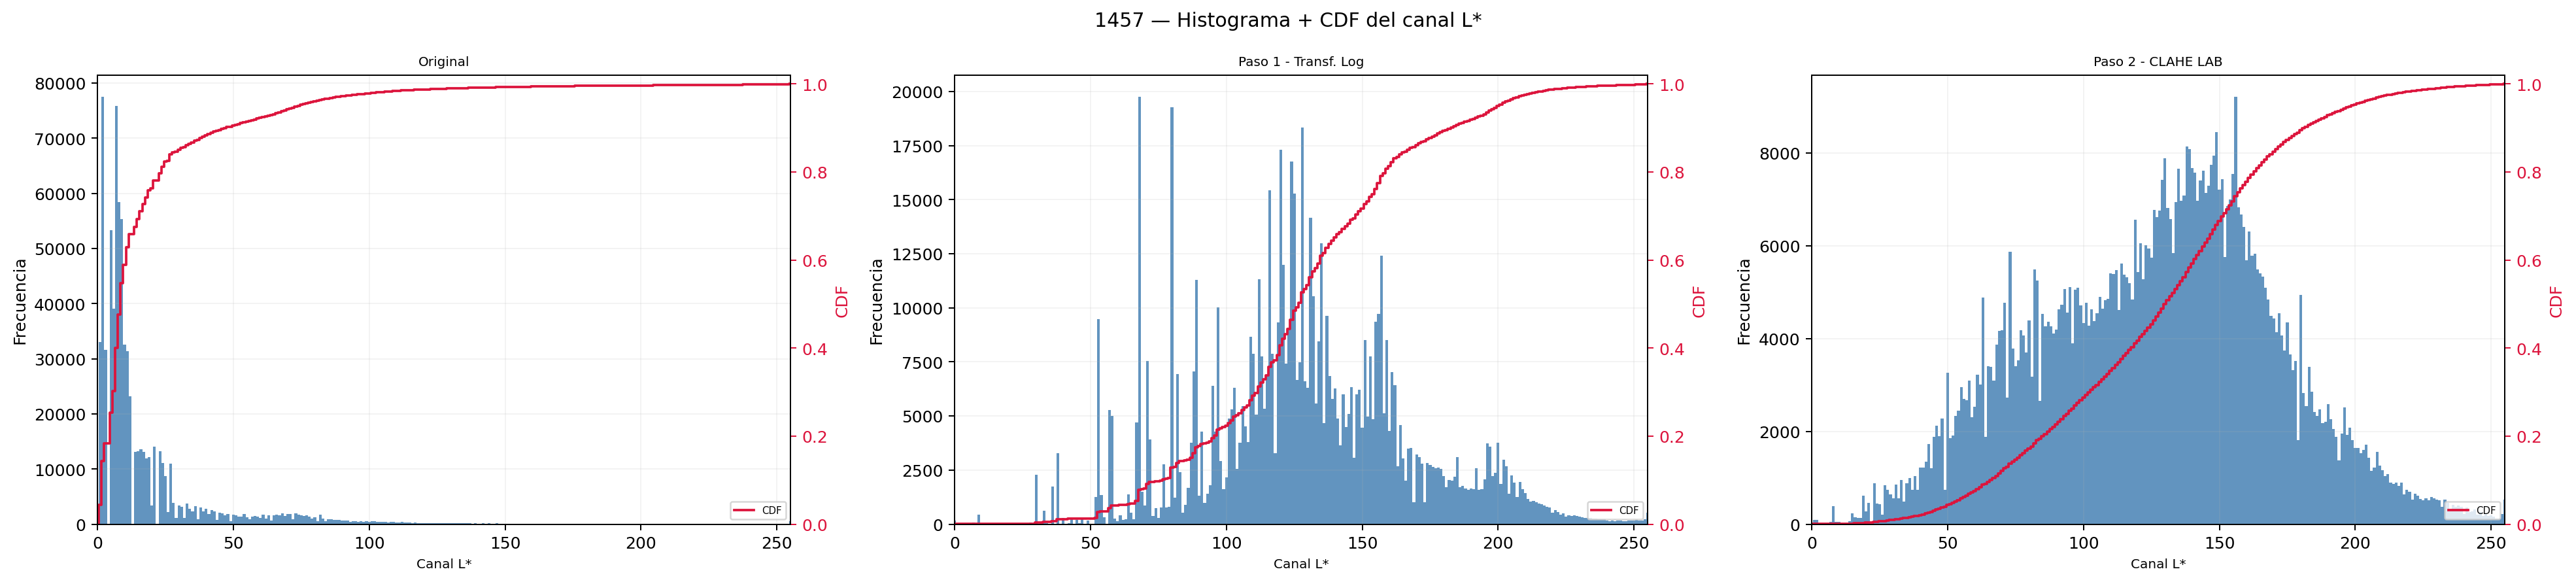
\includegraphics[width=\textwidth]{figures/fig_1457_hist.png}
            \caption{Imagen~1457: histogramas y CDF del canal~$L^*$ por etapa.}
            \label{fig:1457_hist}
        \end{figure}

    \subsection{Imagen 1619: Transformación Logarítmica + CLAHE LAB}

        La imagen~1619 combina zonas de iluminación intermedia, como partes de los coches, 
        con regiones oscuras. Como se aprecia en la Figura~\ref{fig:1619_visual}, la transformación logarítmica expande el
        histograma y permite rescatar la información de los coches y el entorno urbano de la imagen, mientras que el CLAHE LAB introduce una
        mejora local que hace perceptibles detalles de textura previamente
        ocultos. Al igual que en las imágenes anteriores, la etapa CLAHE
        introduce un grano fino en las regiones más oscuras. La Figura~\ref{fig:1619_hist} confirma este efecto mediante una redistribución más amplia.

        \begin{figure}[t]
            \centering
            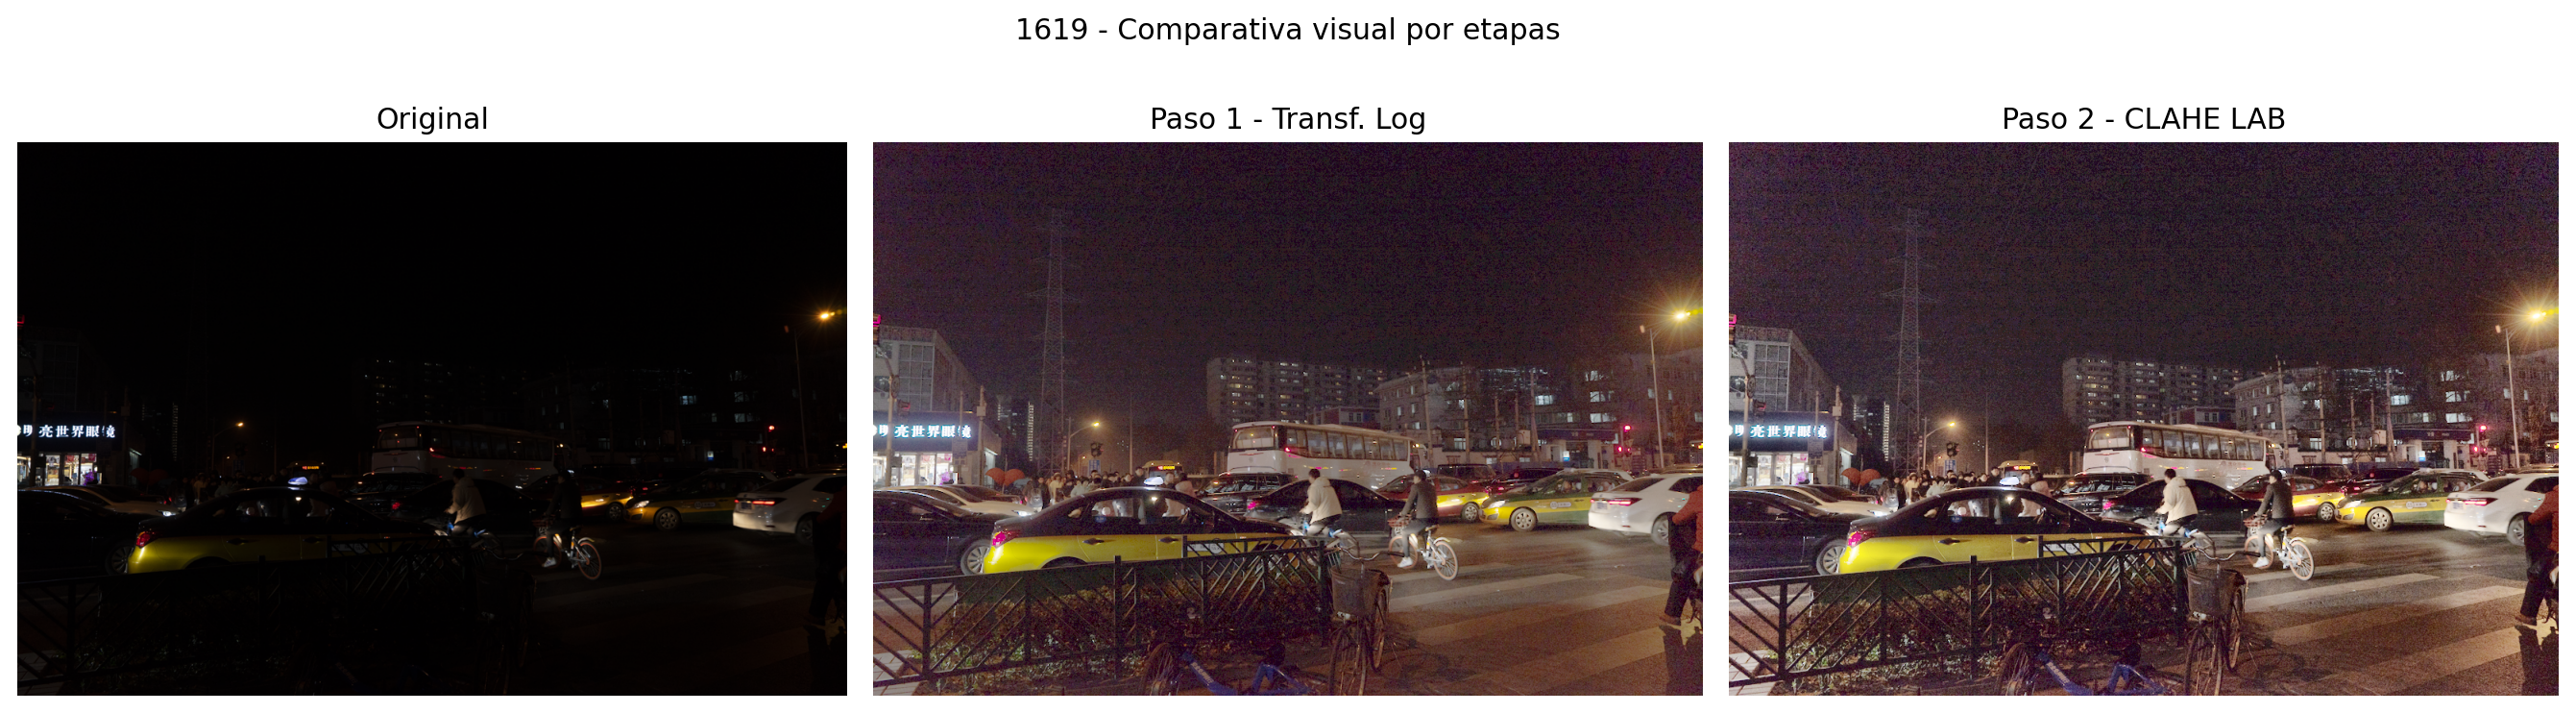
\includegraphics[width=\textwidth]{figures/fig_1619_visual.png}
            \caption{Imagen~1619: comparativa visual por etapa. De izquierda a
            derecha: original, transformación logarítmica y
            CLAHE LAB, clip\,=\,2{,}0, tile\,=\,$8\times8$.}
            \label{fig:1619_visual}
        \end{figure}

        \begin{figure}[t]
            \centering
            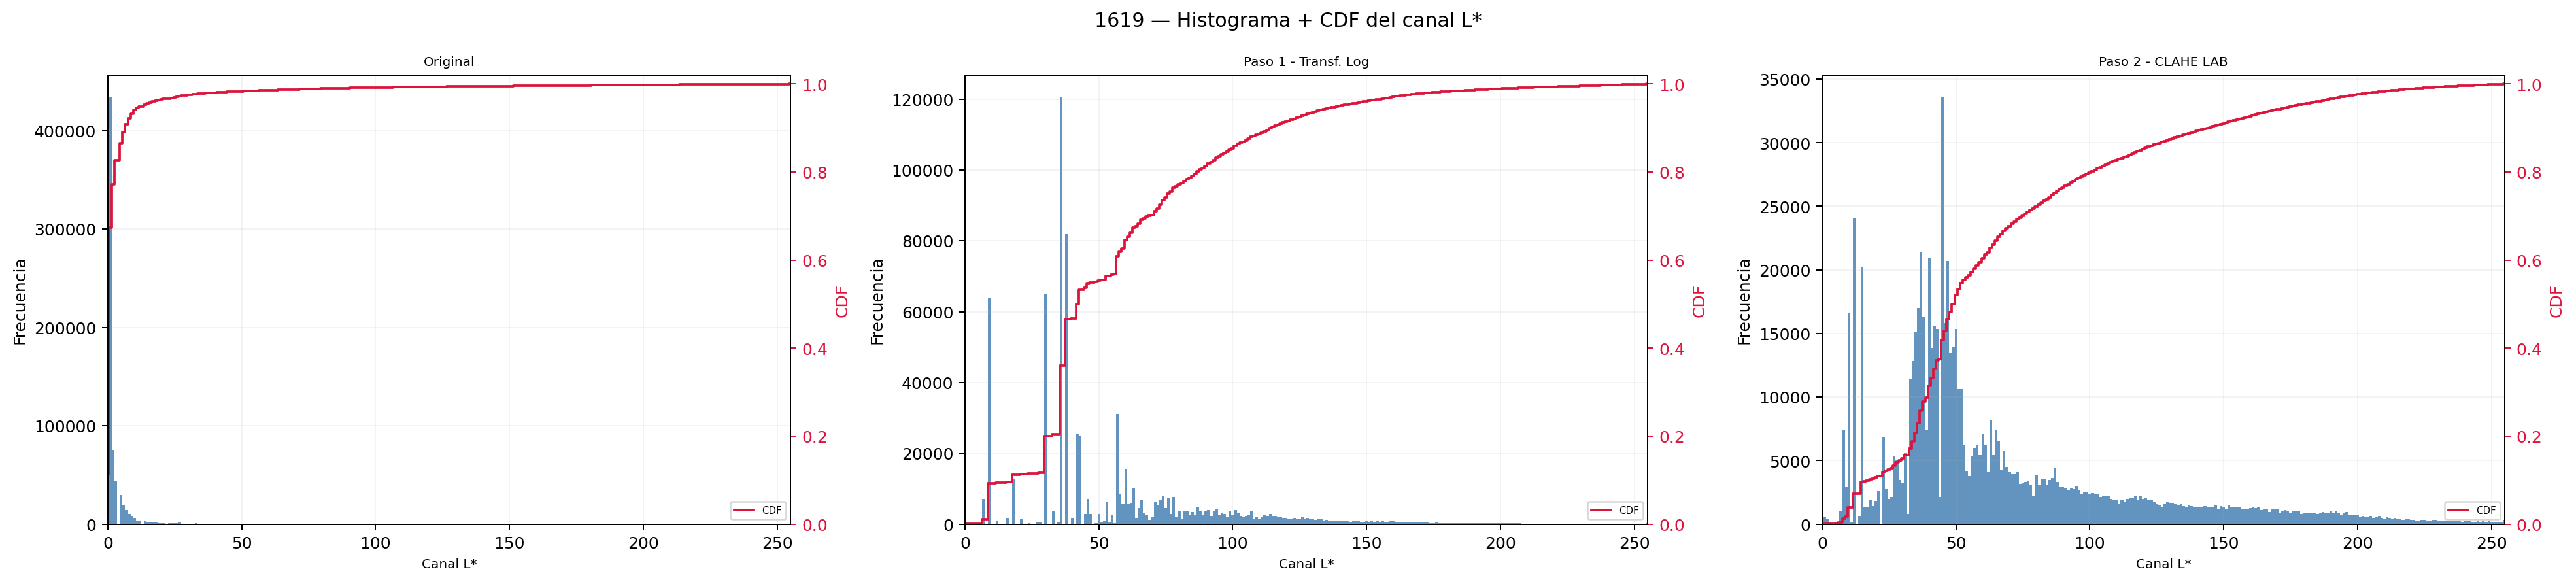
\includegraphics[width=\textwidth]{figures/fig_1619_hist.png}
            \caption{Imagen~1619: histogramas y CDF del canal~$L^*$ por etapa.}
            \label{fig:1619_hist}
        \end{figure}

    \FloatBarrier

%----------------------------------------------------------

\section{Conclusiones}

    Los resultados obtenidos muestran que el flujo de mejora en dos etapas,
    basado en un ajuste de intensidad seguido de CLAHE LAB,
    es capaz de incrementar enormemente la calidad visual de imágenes
    nocturnas de baja iluminación, tal como se aprecia en la inspección
    comparativa de imágenes, histogramas y CDF.

    En cuanto a la eficacia de cada técnica, la aplicación de la ley de potencia resulta
    idónea para imágenes con distribución de intensidades extremadamente
    concentrada en el extremo oscuro (imagen~1187), gracias a su capacidad de
    expandir de forma agresiva los tonos muy bajos. No obstante, esta agresividad
    conlleva la limitación más relevante observada: la saturación y el
    efecto de halo que se ve en los bordes de la imagen, que es una
    consecuencia directa del uso de valores de $\gamma$ muy reducidos en escenas
    con iluminación extremadamente baja. Para las imágenes con mayor variedad tonal
    (1321, 1457 y 1619), la transformación logarítmica ofrece un realce más
    suave y controlado que evita la sobreexposición, siendo preferible en
    presencia de fuentes de luz visibles.

    La aplicación de CLAHE LAB como segunda etapa aporta mejoras consistentes
    en todos los casos, al redistribuir el contraste de forma adaptativa sin
    alterar la cromaticidad de la imagen. Su principal limitación es la
    introducción de ruido en las regiones de muy baja luminancia.

    Como líneas de mejora futura, se propone: (i)~la optimización automática
    del parámetro $\gamma$; (ii)~la incorporación de una etapa de reducción
    de ruido previa o posterior al CLAHE para mitigar el efecto de grano;
    y (iii)~la exploración de métodos de mejora más avanzados, como las redes
    convolucionales entrenadas específicamente en conjuntos de datos de
    escenas nocturnas como \textit{DARK FACE}~\parencite{yang2020darkface}.

%----------------------------------------------------------

\section*{Declaración sobre el uso de IA}
\addcontentsline{toc}{section}{Declaración sobre el uso de IA}

    En la elaboración del presente informe se han utilizado las siguientes
    herramientas de inteligencia artificial:

    \begin{itemize}
        \item \textbf{NotebookLM}: empleado como asistente de
        consulta sobre el temario de la asignatura. Se utilizó para formular
        preguntas sobre conceptos teóricos del procesamiento digital de imágenes
        como transformaciones de intensidad, ecualización de histograma, 
        y contrastar su comprensión con los materiales
        proporcionados por el profesorado. En ningún caso se delegó en esta
        herramienta la redacción de contenidos ni la interpretación de resultados
        experimentales. También fue útil para acelarar la comprensión de los artículos 
        científicos citados en este informe.

        \item \textbf{GitHub Copilot}: utilizado en dos
        contextos diferenciados. Por un lado, como asistente de edición durante la
        maquetación del documento en \LaTeX{}, para tareas de formato
        como estructura de tablas, ajuste de entornos y corrección de
        errores de compilación. Además, se utilizó como apoyo en el
        desarrollo del cuaderno de laboratorio (Jupyter Notebook), asistiendo en
        la creación de funciones auxiliares de visualización, exportación de
        figuras y resolución de errores de ejecución. En ambos usos, la lógica del
        flujo de procesamiento, la selección de parámetros y la interpretación
        de los resultados son de autoría propia inspirados en el código proporcionado en el campus virtual.
    \end{itemize}

%----------------------------------------------------------

\printbibliography

%----------------------------------------------------------

\end{document}
